\section{Experiments}
\label{sec:experiments}
In this section, we evaluate our method using  TU-Berlin sketch benchmark. It contains 250 classes. Each class has 80 instances. We do a group of experiments to compare our method with other methods in recognition speed and accuracy. Like previous works, we use 3-fold cross-validation within the dataset.  We use sketch dataset augmentation scenario  ~\cite{Yu2015SketchaNetTB} to ease our over-fitting problem(see Fig ~\ref{fig:aug_data}).

\begin{figure}[htbp]
    \center
    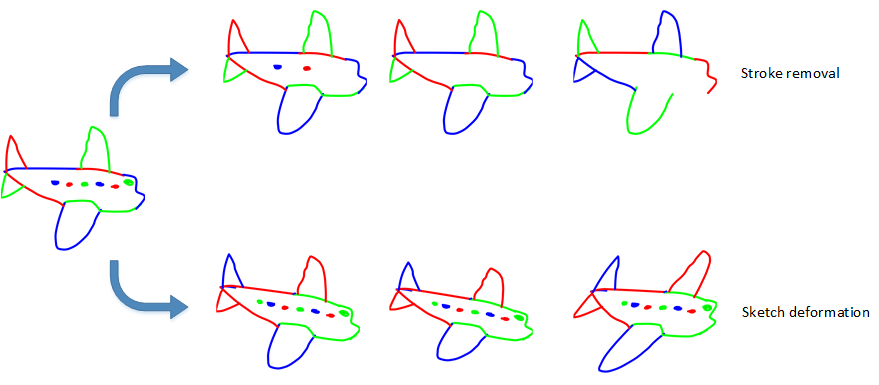
\includegraphics[width=3in]{images/aug_data.png}
    \fcaption{Sketch data augmentation.}
    \label{fig:aug_data}
\end{figure}

\subsection{Recognition accuracy with different $N$}
\label{ssec:resample_number}

From the Fig.~\ref{fig:resample}, we can see that 1024 points are enough to represent a tree. 512 points can also represent a tree but a little sparser. Even a tree with 256 points are visually clear for humans. In order find a proper $N$, we did a group experiments with $N = 1024, 512, 256, 128$. If $N$ is too large, there are no good for recognition accuracy, but makes recognition speed slower.

\begin{table}[htbp]
\begin{tabular}{|p{1.4cm}|p{1.3cm}|p{1.3cm}|p{1.3cm}|p{1.3cm}|}
    \hline
     $N$ & 1024& 512 & 256 & 128\\
    \hline
     accuracy & x\% & x\% & x\%& x\%\\
    \hline
     time & x & x & x& x\\
    \hline
\end{tabular}
\caption{Classification with different $N$.}
\end{table}

\subsection{Comparison of different methods in recognition speed and accuracy}
\label{ssec:cm_speed}
SketchPointNet is derived from PointNet. It uses lots of shared architecture, which means less parameters compared with existing Image-based sketch recognition approaches. We performed Sketch-a-Net(vallina), DeepSketch 1 and SketchPointNet on Titan 1080 with tensorflow 1.2. The whole model of Sketch-a-Net and DeepSketch 2 \cite{Dupont2016DeepSketch2D} use different feature fusion method, which makes the whole models too large to suite the mobile computing device. So we only compare 3 end-to-end networks(Sketch-a-Net(vallina), DeepSketch 1 and SketchPointNet).

\begin{table}[htbp]
\centering
\footnotesize
\begin{tabular}{cccc}
    \hline
     -&Sketch-a-Net(vallina)& DeepSketch 1& Ours\\
    \hline
     model size& 64M&223M& 33M\\
     speed &10.9ms&10.6ms& 4.1ms\\
     total feature maps& 79w& 128.4w& 698.1w\\
     trainable parameters&824w& 5510w& 64.86w\\
    \hline
\end{tabular}
\caption{Performance comparison of different networks(gpu).}
\label{tbl:speed}
\end{table}




\begin{table*}
\centering
\small
\begin{tabular}{lllll}
    \hline
     models&group parameters& time/sketch& accuracy &memory\\
    \hline
     SketchPointNet1(mlp(8,16,64), mlp(32,32,128), mlp(64,128,1024))&group1(512*30), group2(256*100)& 163.8ms& 73.5\% & 3.11G\\
    \hline
     Sketch-a-Net& - &82.7ms& 77.9\% & 529M\\
    \hline
     DeepSketch 1& - &106.3ms& 75.42\% & 573M\\
    \hline
\end{tabular}
\caption{Performance comparison of different networks(cpu).}
\label{tbl:speed_cpu}
\end{table*}

\begin{table*}
\centering
\begin{tabular}{llll}
    \hline
     models&group parameters& accuracy& stroke order\\
    \hline
     SketchPointNet(mlp(8,16,64), mlp(32,32,128), mlp(64,128,1024))&group1(512*30), group2(256*100)& 73.5\% & y\\
    \hline
     SketchPointNet(mlp(8,16,64), mlp(32,32,128), mlp(64,128,1024))&group1(512*30), group2(256*100)& 69.6\% & n\\
    \hline
     PointNet++(mlp(8,16,64), mlp(32,32,128), mlp(64,128,1024))&group1(512*30), group2(256*100)& 51.2\% &n\\
    \hline
     PointNet++(mlp(64,64,128), mlp(128,128,256), mlp(256,512,1024))&group1(512*64), group2(128*64)& 58.7\% &n\\
    \hline
     PointNet(mlp(64,64,64,128,1024))&-& 46\% &n\\
    \hline
\end{tabular}
\caption{Comparing with PointNet and PointNet++}
\label{tbl:pointnet_cp}
\end{table*}

From the tabel ~\ref{tbl:speed} we can see that our model is faster and smaller than Sketch-a-Net(vallina) and DeepSketch 1. Although our model are smaller compared with existing DNN-based appraches. We still achieve a high recognition accuracy.

\begin{table}[htbp]
\centering
\begin{tabular}{lc}
    \hline
     models &accuracy\\
    \hline
     HOG-SVM ~\cite{Eitz2012HowDH}& 56\% \\
     MKL-SVM ~\cite{LiHSG15} & 65.8\% \\
     FV-SP ~\cite{Schneider2014SketchCA} & 68.9\% \\
     LeNet ~\cite{LeCun1998GradientbasedLA}& 55.2\% \\
     Sketch-a-Net(vallina) ~\cite{Yu2015SketchaNetTB}& 72.6\% \\
     Sketch-a-Net ~\cite{Yu2015SketchaNetTB}& 77.95\% \\
     DeepSketch 1 ~\cite{Seddati2015DeepSketchDC}& 75.42\% \\
     DeepSketch 2 ~\cite{Dupont2016DeepSketch2D}& 77.69\% \\
     PointNet ~\cite{qi2017pointnet}& 46\% \\
     PointNet++ ~\cite{qi2017pointnetplusplus}& 58.7\% \\
     Our Model& 73.5\% \\
    \hline
\end{tabular}
\caption{Sketch recognition with different models.}
\label{tbl:acc}
\end{table}

Fig. ~\ref{fig:resshow} shows some results. Although our network can handle some challenging cases(green). SketchPointNet still fail on very ambiguous cases(the reds are predictions, the blacks are ground truth for each case).

\begin{figure}[htbp]
    \center
    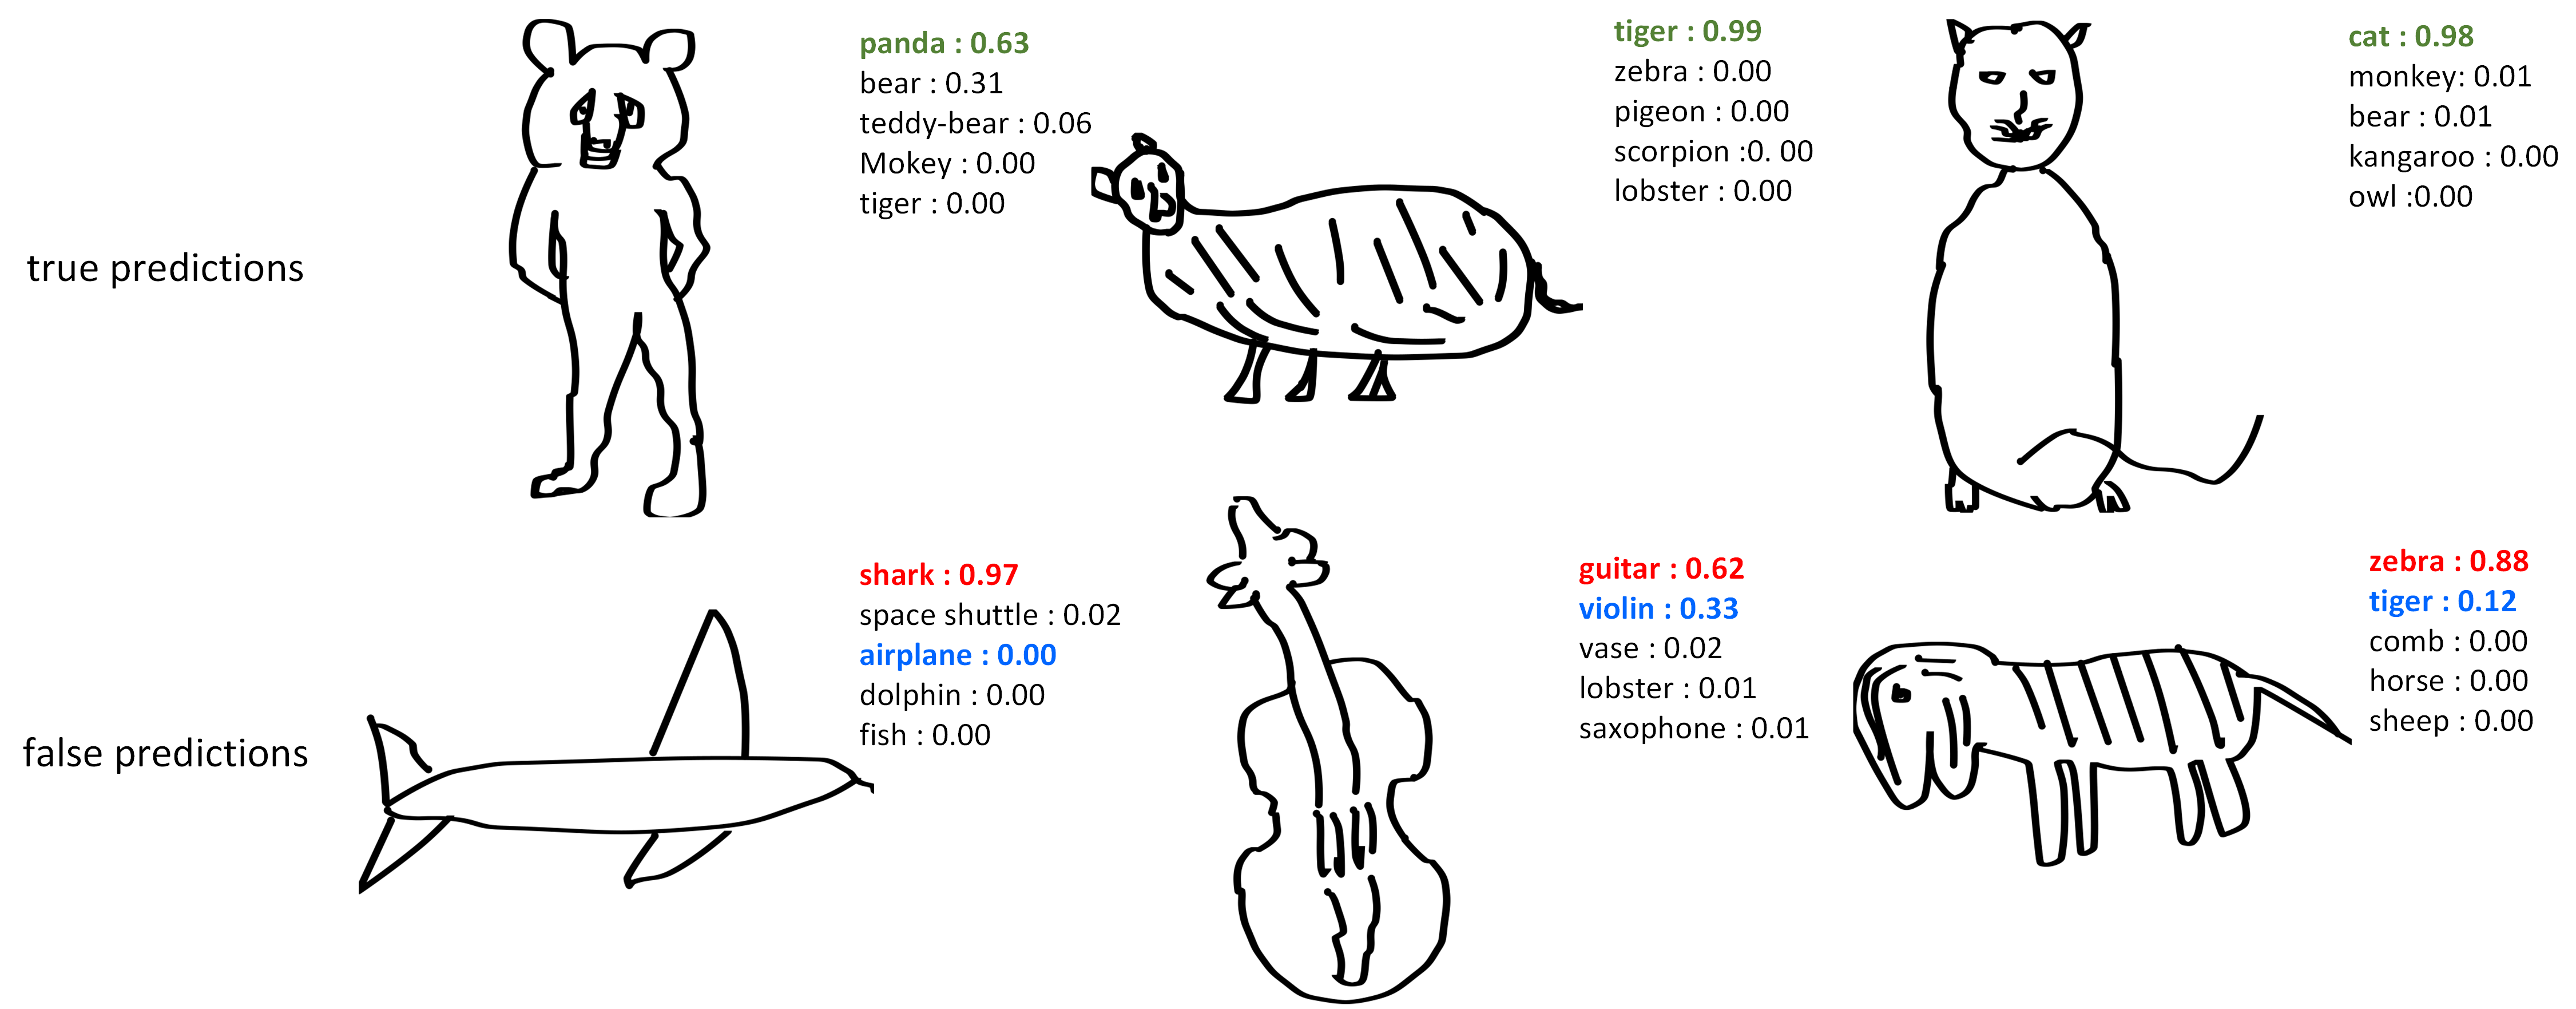
\includegraphics[width=3in]{images/res.png}
    \fcaption{Illustration of recognition successes (green) and failures (red).}
    \label{fig:resshow}
\end{figure}
